\begin{frame}[fragile]{Concepto del perfilador}
    \begin{onlyenv}<1>
        \begin{columns}
            \begin{column}{0.5\textwidth}
            
                \begin{itemize}
                    \item Determinar el perfil especial del haz en un plano
                    \item Al desplazarse permite determina la divergencia del haz.
                    \item Perfiladores con cámaras CCD. Sensores muy caros
                    \item Perfiladores integradores. Complejidad mecánica
                \end{itemize}
            \end{column}
            
            \begin{column}{0.5\textwidth}
                \begin{figure}[H]
                \centering
                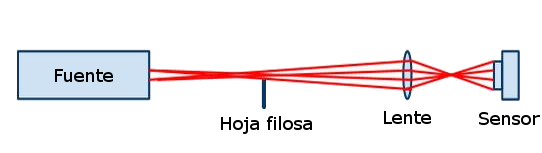
\includegraphics[width=\textwidth]{fig/perfilador/esquema_basico}
                \label{fig:perfilador/esquema_basico}
                \end{figure}
            \end{column}
        \end{columns}
    \end{onlyenv}

    \begin{onlyenv}<2>
        \centering
        Para haces gaussianos (\underline{la mayoría}), el perfil de intensidades, es decir la integral del perfil, es la función error

        \begin{figure}
            \centering
            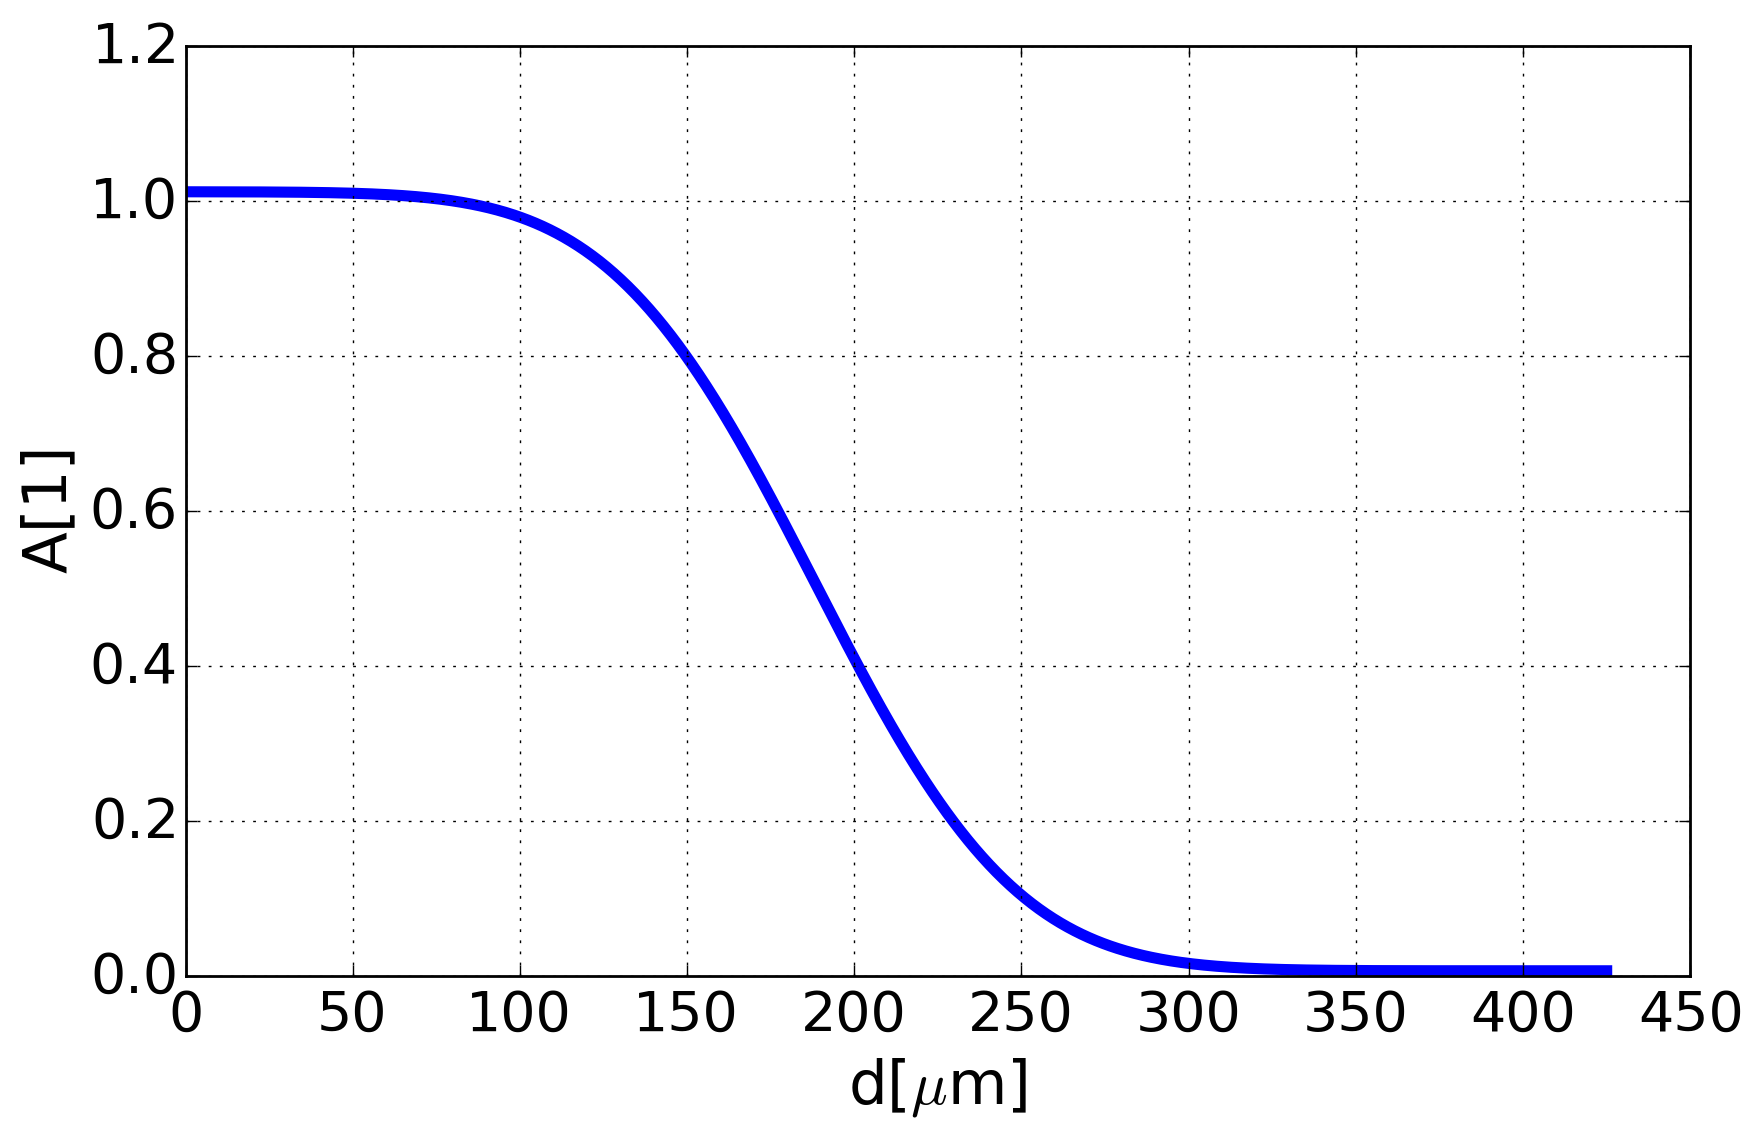
\includegraphics[width=0.8\textwidth]{fig/perfilador/err_function.png}
            \label{fig:perfilador/err_function}
        \end{figure}

    \end{onlyenv}

\end{frame}

\begin{frame}[fragile]{Concepto del polarizador}
    \begin{onlyenv}<1>
        \begin{figure}[H]
            \centering
            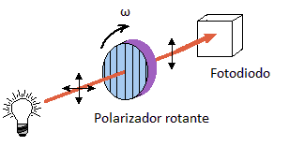
\includegraphics[width=0.4\textwidth]{fig/polarimetro/esquema}
            %\caption{}
            \label{fig:polarimetro}
        \end{figure}
        \begin{itemize}
            \item Permite determinar eje mayor y eje menor de polarización eliptica. 
            \item Permite identificar polarización circular.
            \item Depende de la precisión de rotación del motor, pero puede mejorarse con mecánica adecuada.
        \end{itemize}
    \end{onlyenv}
    \begin{onlyenv}<2>
        \centering
        Ley de Malus
        \begin{figure}[H]
            \centering
            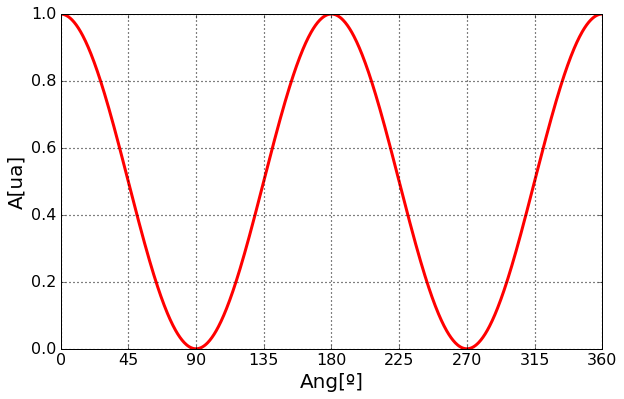
\includegraphics[width=0.6\textwidth]{fig/polarimetro/malus}
            %\caption{}
            \label{fig:polarimetro}
        \end{figure}
        \[ \alpha = \frac{\max - \min}{\max + \min} = \begin{cases} 1 & \text{si lineal} \\ 0 & \text{si circular} \\ (0, 1) & \text{si eliptica} \end{cases}\]
    \end{onlyenv}
\end{frame}
